%% IEEE Conference Paper — ST-GAT IDS for V2X
%% Author: Mostafa Mohamed Atef et al. — E-JUST 2026
%% Compile: pdflatex → bibtex → pdflatex × 2

\documentclass[conference]{IEEEtran}
\IEEEoverridecommandlockouts

% ── Packages ─────────────────────────────────────────────────────────────────
\usepackage{cite}
\usepackage{amsmath,amssymb,amsfonts}
\usepackage{algorithm}
\usepackage{algorithmic}
\usepackage{graphicx}
\usepackage{textcomp}
\usepackage{xcolor}
\usepackage{booktabs}
\usepackage{multirow}
\usepackage{array}
\usepackage{tikz}
\usetikzlibrary{shapes.geometric,shapes.multipart,arrows.meta,
                positioning,calc,fit,backgrounds,decorations.pathreplacing}
\usepackage{pgfplots}
\pgfplotsset{compat=1.17}

% ── TikZ styles ──────────────────────────────────────────────────────────────
\tikzset{
  block/.style  = {rectangle, draw, fill=blue!10, rounded corners,
                   minimum width=2.0cm, minimum height=0.6cm,
                   font=\footnotesize, align=center},
  sblock/.style = {rectangle, draw, fill=orange!15, rounded corners,
                   minimum width=2.0cm, minimum height=0.55cm,
                   font=\scriptsize, align=center},
  fuse/.style   = {rectangle, draw, fill=green!12, rounded corners,
                   minimum width=5.2cm, minimum height=0.65cm,
                   font=\footnotesize\bfseries, align=center},
  inp/.style    = {rectangle, draw=gray!60, fill=gray!8, rounded corners,
                   minimum width=2.0cm, minimum height=0.55cm,
                   font=\scriptsize, align=center},
  arr/.style    = {-{Stealth[length=4pt]}, thick},
  darr/.style   = {-{Stealth[length=4pt]}, thick, dashed, gray!60},
}

\def\BibTeX{{\rm B\kern-.05em{\sc i\kern-.025em b}\kern-.08em
    T\kern-.1667em\lower.7ex\hbox{E}\kern-.125emX}}

% ─────────────────────────────────────────────────────────────────────────────
\begin{document}

\title{AI-Driven Behavioural Anomaly Detection for V2X Communications:\\
A Spatio-Temporal Graph Attention Transformer\\with Targeted Fine-Tuning}

\author{
\IEEEauthorblockN{Mostafa Mohamed Atef\textsuperscript{*},
                  Ahmed Fikry\textsuperscript{*},
                  Ebrahim Ramadan Diab\textsuperscript{*},
                  Mazen Mohamed\textsuperscript{*},
                  Kareem Kamel Elfiky\textsuperscript{*},
                  Ahmed Saber Mohamed\textsuperscript{*},
                  Prof.\ Samir A.\ ElSagheer\textsuperscript{*}}
\IEEEauthorblockA{\textsuperscript{*}Faculty of Computer Science and Information Technology,\\
Egypt-Japan University of Science and Technology (E-JUST), Alexandria, Egypt\\
\small\{mostafa.atef, ahmed.fikry, ebrahim.torad, mazen.abohanifa, kareem.elfeky, ahmed.yousef\}@ejust.edu.eg\\
\small samir.elsagheer@ejust.edu.eg}
}

\maketitle

% ── Abstract ─────────────────────────────────────────────────────────────────
\begin{abstract}
Post-quantum cryptographic schemes address the identity-authentication
layer of Vehicle-to-Everything (V2X) security but cannot detect content
falsification by vehicles that hold valid credentials.  We present an
AI-driven Intrusion Detection System (IDS) that provides the complementary
\emph{behavioural} detection layer.  The system is built around a
Spatio-Temporal Graph Attention Transformer (ST-GAT): a four-stream
architecture that processes per-vehicle temporal sequences through a
Transformer encoder (Stream~A), models cross-feature correlations via
iTransformer-style feature attention (Stream~B), captures inter-vehicle
spatial coordination with a two-layer Graph Attention Network (Stream~C),
and directly fingerprints window-level attack signatures through a
hand-crafted aggregate MLP (Stream~D).  Training employs a
vehicle-ID-stratified three-way split to eliminate monitoring-signal
leakage, normal-class upsampling to stabilise class-weight gradients, and
a two-stage protocol: per-attack-type focal-loss weighting in Stage~1
followed by targeted fine-tuning that boosts the hardest residual class
in Stage~2.  Evaluated on the VeReMi NextGen benchmark (619,097 BSMs,
14 attack types, highway scenario), the model achieves
F1\,$=$\,0.9913, Recall\,$=$\,0.9886, ROC-AUC\,$=$\,0.9923,
MCC\,$=$\,0.8699, and Precision\,$=$\,0.9940, with inference latency of
23.4\,ms per sample --- well within the 100\,ms real-time V2X budget.
All 14 attack types are detected; 13 achieve F1\,$\geq\,$0.998 and
\texttt{timeDelayAttack} achieves F1\,$=$\,0.9348 at perfect precision.
\end{abstract}

\begin{IEEEkeywords}
V2X security, intrusion detection system, spatio-temporal graph attention
transformer, targeted fine-tuning, focal loss, VeReMi NextGen, behavioural
anomaly detection, misbehaviour detection, vehicle-stratified split
\end{IEEEkeywords}

% ─────────────────────────────────────────────────────────────────────────────
\section{Introduction}
\label{sec:intro}

Intelligent transportation systems increasingly depend on
Vehicle-to-Everything (V2X) communication for collision avoidance,
cooperative driving, and emergency notification~\cite{boualouache2023survey}.
Each participating vehicle broadcasts Basic Safety Messages (BSMs) at
approximately 10\,Hz, containing GPS position, speed, heading, and
acceleration.  The integrity of this data stream is safety-critical: a
falsified position broadcast can trigger phantom emergency braking
cascades, while a Sybil attack injecting multiple phantom vehicles into
traffic maps can divert platoons into hazards.

The companion work to this paper~\cite{pqascms2025} addresses the
cryptographic authentication layer, proposing a Post-Quantum Aware
Security Credential Management System (PQA-SCMS) that selectively applies
CRYSTALS-Dilithium~\cite{dilithium2021} and Kyber~\cite{kyber2021} to
long-term V2X certificates while retaining ECDSA for bandwidth-constrained
high-frequency messages.  This approach ensures that message
\emph{provenance} is cryptographically verifiable even against quantum
adversaries, achieving 100\% detection of replay and signature-forgery
attacks.

However, cryptographic authentication is a necessary but not sufficient
condition for V2X safety.  A vehicle holding a valid post-quantum
credential can still broadcast physically implausible data---falsified GPS
coordinates, impossible accelerations, or artificially delayed messages.
Content falsification demands \emph{behavioural} detection: analysis of
whether the reported physics of vehicle motion are internally consistent,
temporally plausible, and spatially coherent relative to nearby vehicles.

Existing V2X IDS approaches fall into three categories.
\emph{Rule-based} systems~\cite{vanderheijden2018veremi} apply handcrafted
kinematic thresholds to individual messages, failing on attacks that are
individually plausible but collectively anomalous across time or space.
\emph{Classical ML} methods~\cite{gyawali2020challenges} (SVMs, random
forests) capture statistical patterns but discard temporal dependencies and
inter-vehicle relationships.  \emph{Deep learning} approaches improve
detection but typically address a narrow subset of attack types or treat
BSMs as independent samples, ignoring the spatio-temporal structure that
encodes the most discriminative signals for coordinated attacks.

\textbf{Contributions.}  This paper makes four contributions:
\begin{enumerate}
\item A four-stream ST-GAT architecture that simultaneously models temporal
  vehicle dynamics (Stream~A), feature cross-correlations (Stream~B),
  multi-vehicle spatial coordination (Stream~C), and explicit window-level
  attack fingerprints (Stream~D), achieving complementary coverage of all
  14 VeReMi NextGen attack types in a single unified model.
\item A vehicle-ID-stratified three-way train/val/test split paired with
  normal-class upsampling that eliminates monitoring-signal leakage and
  reduces the effective class weight from 14.6$\times$ to $\approx$3$\times$.
\item A vectorised O(1) spatial neighbour index based on integer-hash
  encoding that avoids the memory and compute cost of a full cross-join
  over 619,097 messages.
\item A comprehensive evaluation demonstrating MCC\,$=$\,0.870 on a
  93.6\%-attack dataset, confirming genuine discriminative ability beyond
  majority-class exploitation, alongside 23.4\,ms inference latency
  compatible with real-time V2X deployment.
\end{enumerate}

% ─────────────────────────────────────────────────────────────────────────────
\section{Related Work}
\label{sec:related}

\subsection{Rule-Based and Statistical Misbehaviour Detection}

The VeReMi dataset~\cite{vanderheijden2018veremi} and its NextGen
extension~\cite{kamel2020veremi} are the primary V2X IDS benchmarks.
Early detection work applied position-plausibility checks and kinematic
consistency thresholds, achieving high recall on simple offset attacks
while failing on temporally subtle ones such as \texttt{timeDelayAttack},
which requires analysis of gap patterns across multiple consecutive
messages.  Gyawali et al.~\cite{gyawali2020challenges} survey the
challenge space, identifying sensor fusion, privacy constraints, and
signal ambiguity between attack-induced and noise-induced anomalies as
open problems.

\subsection{Deep Learning for V2X Anomaly Detection}

Convolutional and recurrent models have been applied to per-vehicle BSM
streams.  LSTM-based encoders~\cite{ercan2022misbehavior} capture temporal
dynamics of individual vehicles, improving recall on timing attacks but
providing limited coverage of spatially-coordinated attacks such as
\texttt{trafficCongestionSybil}, which requires multi-vehicle context.
Transformer encoders~\cite{vaswani2017attention} have demonstrated strong
performance on sequential anomaly detection across domains, yet their
application to multi-type V2X attack detection with explicit graph
structure has not been previously reported.

\subsection{Graph Neural Networks for Vehicular Networks}

Graph-based approaches~\cite{velickovic2018gat} are natural for V2X given
the vehicular network's inherent spatial topology.  Ko et
al.~\cite{ko2020vcn} apply spectral graph convolutions to static road
graphs.  Our approach differs by constructing a dynamic per-sample
neighbourhood graph from real-time spatial proximity, directly enabling
detection of Sybil coordination where multiple phantom vehicles broadcast
from the same spatial cell simultaneously.

\subsection{iTransformer for Multivariate Signals}

The iTransformer~\cite{itransformer2024} inverts the conventional
Transformer by treating feature dimensions as tokens rather than time
steps, explicitly learning cross-feature correlations.  We adopt this
paradigm for Stream~B to capture the correlated nature of BSM sensor
fields, where anomalous co-variation across position, speed, and noise
channels is more informative than any single feature in isolation.

% ─────────────────────────────────────────────────────────────────────────────
\section{Problem Formulation}
\label{sec:problem}

\subsection{BSM Data Model}

Let $\mathcal{V} = \{v_1, \ldots, v_N\}$ denote active vehicles in a V2X
scenario.  Each vehicle $v$ transmits a BSM stream
$\mathcal{M}_v = \{m_{v,t}\}_{t=1}^{T_v}$, where
$m_{v,t} \in \mathbb{R}^{d}$ comprises $d_{\text{raw}}=10$ raw sensor
fields extended to $d'=15$ by the engineered features of
Section~\ref{sec:features}.  A \emph{temporal window} of size $W=20$
centred at time $t$ is
$\mathbf{X}_{v,t} = [m_{v,t-W+1}, \ldots, m_{v,t}] \in \mathbb{R}^{W \times d'}$.

\subsection{Spatial Neighbourhood}

The neighbourhood of vehicle $v$ at time $t$ is:
\begin{equation}
\mathcal{N}(v,t) = \bigl\{u \in \mathcal{V} \setminus \{v\} \mid
  \|\mathbf{p}_u - \mathbf{p}_v\| \leq \delta,\;
  |t_u - t_v| \leq \tau \bigr\}
\end{equation}
with spatial radius $\delta=300$\,m and temporal tolerance $\tau=0.5$\,s,
capped at $K=8$ deduplicated neighbours.

\subsection{Detection Objective}

Given a window $\mathbf{X}_{v,t}$, neighbour windows
$\{\mathbf{X}_{u,t}\}_{u \in \mathcal{N}(v,t)}$, and a window aggregate
vector $\mathbf{w}_{v,t} \in \mathbb{R}^8$, the IDS produces:
\begin{equation}
\hat{y}_{v,t} = \mathbf{1}\!\left[\hat{p}_{v,t} \geq \theta\right],
\quad
\hat{p}_{v,t} = f_\phi\!\left(\mathbf{X}_{v,t},
  \{\mathbf{X}_{u,t}\},
  \mathbf{w}_{v,t}\right)
\end{equation}
where $f_\phi$ is the ST-GAT with parameters $\phi$ and $\theta$ is the
operating threshold chosen post-training on the validation set.

\subsection{Attack Taxonomy}

The 14 attack types in VeReMi NextGen span five categories:
\emph{position falsification} (constantPositionOffset,
randomPositionOffset, positionMirroring);
\emph{speed falsification} (randomSpeedOffset, zeroSpeedReport,
suddenConstantSpeed, suddenStop);
\emph{kinematic inconsistency} (feignedBraking,
accelerationMultiplication, reversedHeading);
\emph{timing manipulation} (timeDelayAttack, dataReplay);
\emph{volume DoS} (dosAttack); and
\emph{Sybil coordination} (trafficCongestionSybil).
These categories differ fundamentally in which signal modality is
diagnostic, motivating the multi-stream design.

% ─────────────────────────────────────────────────────────────────────────────
\section{Dataset and Feature Engineering}
\label{sec:features}

\subsection{VeReMi NextGen}

VeReMi NextGen~\cite{kamel2020veremi} provides 619,097 BSMs from a
SUMO-simulated highway (624\,m $\times$ 2,560\,m) with UTM-like metre
coordinates.  Table~\ref{tab:dataset} summarises the split statistics
after windowing ($W=20$, $S=3$) with the vehicle-ID-stratified three-way
split.

\begin{table}[t]
\centering
\caption{Windowed Dataset Statistics (stride $S=3$, $W=20$,
         vehicle-ID-stratified split)}
\label{tab:dataset}
\setlength{\tabcolsep}{4pt}
\begin{tabular}{lrrl}
\toprule
\textbf{Split} & \textbf{Senders} & \textbf{Windows} & \textbf{Note} \\
\midrule
Training & ${\approx}303$ & ${\approx}122{,}047$ & After upsampling \\
Val      & ${\approx}34$  & ${\approx}13{,}554$  & No sender overlap \\
Test     & ${\approx}85$  & ${\approx}33{,}925$  & Held-out final eval \\
\midrule
Total    & ${\approx}422$ & ${\approx}169{,}526$ & \\
\bottomrule
\end{tabular}
\end{table}

The 93.6\% attack ratio arises from the labelling scheme: every window
drawn from any non-normal (sender\_id, attack\_type) group receives
$y=1$, including victim-vehicle windows in the trafficCongestionSybil
scenario.  This makes the Matthews Correlation Coefficient (MCC), rather
than accuracy or F1, the primary reliability metric.

\subsection{Raw Features}

The 10 raw BSM fields are: UTM position $(x, y)$, speed~$v$,
heading~$\phi$, acceleration~$a$, inter-message gap~$\Delta t$, and four
noise-magnitude channels $(\eta_x, \eta_v, \eta_\phi, \eta_a)$.

\subsection{Physics-Based Engineered Features}

Five consistency metrics are computed from per-vehicle consecutive message
differences:

\textbf{Kinematic error} measures how far the reported GPS position
deviates from the kinematic model prediction:
\begin{equation}
e_{\text{kin},t} =
  \bigl\|\Delta\mathbf{p}_t - v_{t-1}\hat{\mathbf{d}}_{t-1}\Delta t\bigr\|_2
\end{equation}

\textbf{Speed consistency} compares position-implied speed to reported
speed:
\begin{equation}
e_{\text{spd},t} = \left|\frac{\|\Delta\mathbf{p}_t\|}{\Delta t} - v_t\right|
\end{equation}

\textbf{Heading consistency} measures the angular deviation between
actual movement direction and reported heading:
\begin{equation}
e_{\text{hed},t} = \min(\theta_t,\, 2\pi - \theta_t),\quad
\theta_t = \bigl(\phi^{\text{move}}_t - \phi^{\text{rep}}_t\bigr)
           \bmod 2\pi
\end{equation}

\textbf{Acceleration consistency} compares speed-delta acceleration to
reported acceleration:
\begin{equation}
e_{\text{acl},t} = \left|\frac{v_t - v_{t-1}}{\Delta t} - a_t\right|
\end{equation}

\textbf{Spatial density} counts unique vehicle IDs in the same
$\delta\,\times\,\delta$ cell ($\delta=300$\,m) per $\tau=0.5$\,s bin,
using the same grid parameters as the spatial index.
All engineered features are clipped to $[0, 10^4]$.

\subsection{Window Aggregate Features (Stream D Input)}

Eight window-level statistics are computed from z-scored sequences and
fed as direct attack fingerprints to Stream~D:
\begin{equation}
\mathbf{w} =
\bigl[\max,\sigma,\mu\bigr]_{\Delta t} \oplus
\bigl[\max\bigr]_{e_\text{kin}} \oplus
\bigl[\max\bigr]_{\eta_x} \oplus
\bigl[\max\bigr]_{e_\text{acl}} \oplus
\bigl[\max\bigr]_{e_\text{hed}} \oplus
\bigl[\max\bigr]_{\rho}
\end{equation}
where $\rho$ denotes spatial density.  Computing $\max(\Delta t)$
explicitly reduces the timeDelayAttack detection task from discovering a
temporal pattern to learning a threshold.

% ─────────────────────────────────────────────────────────────────────────────
\section{ST-GAT Architecture}
\label{sec:arch}

\begin{figure}[t]
\centering
\resizebox{\columnwidth}{!}{%
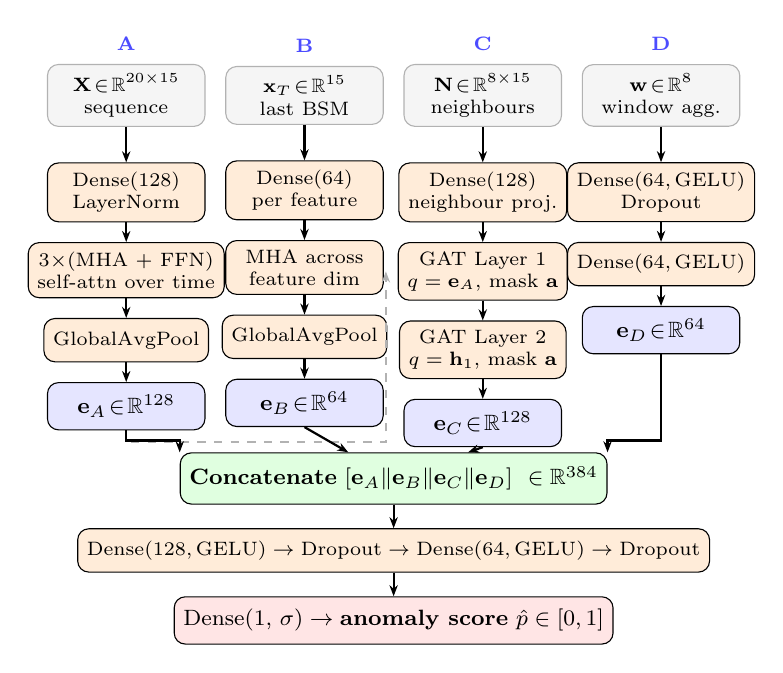
\begin{tikzpicture}[node distance=0.35cm and 0.3cm]

%% ── Inputs ────────────────────────────────────────────────────────────────
\node[inp] (inA) {$\mathbf{X}\!\in\!\mathbb{R}^{20\times15}$\\sequence};
\node[inp, right=0.25cm of inA] (inB) {$\mathbf{x}_T\!\in\!\mathbb{R}^{15}$\\last BSM};
\node[inp, right=0.25cm of inB] (inC) {$\mathbf{N}\!\in\!\mathbb{R}^{8\times15}$\\neighbours};
\node[inp, right=0.25cm of inC] (inD) {$\mathbf{w}\!\in\!\mathbb{R}^{8}$\\window agg.};

%% ── Stream labels ─────────────────────────────────────────────────────────
\node[above=0.05cm of inA, font=\scriptsize\bfseries, color=blue!70] {A};
\node[above=0.05cm of inB, font=\scriptsize\bfseries, color=blue!70] {B};
\node[above=0.05cm of inC, font=\scriptsize\bfseries, color=blue!70] {C};
\node[above=0.05cm of inD, font=\scriptsize\bfseries, color=blue!70] {D};

%% ── Stream A ──────────────────────────────────────────────────────────────
\node[sblock, below=0.45cm of inA] (projA) {Dense(128)\\LayerNorm};
\node[sblock, below=0.25cm of projA] (tfA)  {3$\times$(MHA + FFN)\\self-attn over time};
\node[sblock, below=0.25cm of tfA]  (poolA) {GlobalAvgPool};
\node[block,  below=0.25cm of poolA](embA)  {$\mathbf{e}_A\!\in\!\mathbb{R}^{128}$};

%% ── Stream B ──────────────────────────────────────────────────────────────
\node[sblock, below=0.45cm of inB] (projB) {Dense(64)\\per feature};
\node[sblock, below=0.25cm of projB] (tfB) {MHA across\\feature dim};
\node[sblock, below=0.25cm of tfB]  (poolB){GlobalAvgPool};
\node[block,  below=0.25cm of poolB](embB) {$\mathbf{e}_B\!\in\!\mathbb{R}^{64}$};

%% ── Stream C ──────────────────────────────────────────────────────────────
\node[sblock, below=0.45cm of inC] (projC) {Dense(128)\\neighbour proj.};
\node[sblock, below=0.25cm of projC] (gat1){GAT Layer 1\\$q=\mathbf{e}_A$, mask $\mathbf{a}$};
\node[sblock, below=0.25cm of gat1] (gat2) {GAT Layer 2\\$q=\mathbf{h}_1$, mask $\mathbf{a}$};
\node[block,  below=0.25cm of gat2] (embC) {$\mathbf{e}_C\!\in\!\mathbb{R}^{128}$};

%% ── Stream D ──────────────────────────────────────────────────────────────
\node[sblock, below=0.45cm of inD] (fc1D) {Dense(64,\,GELU)\\Dropout};
\node[sblock, below=0.25cm of fc1D](fc2D) {Dense(64,\,GELU)};
\node[block,  below=0.25cm of fc2D](embD) {$\mathbf{e}_D\!\in\!\mathbb{R}^{64}$};

%% ── Fusion ────────────────────────────────────────────────────────────────
\node[fuse, below=0.5cm of $(embB)!0.5!(embC)$]
  (concat) {Concatenate\;$[\mathbf{e}_A \| \mathbf{e}_B \| \mathbf{e}_C \| \mathbf{e}_D]$\;\;$\in\mathbb{R}^{384}$};

\node[sblock, below=0.3cm of concat, minimum width=5.0cm]
  (fc1) {Dense(128,\,GELU)\;$\to$\;Dropout\;$\to$\;Dense(64,\,GELU)\;$\to$\;Dropout};

\node[block, below=0.3cm of fc1, fill=red!10, minimum width=3.0cm]
  (out) {Dense(1, $\sigma$)\;$\to$\;\textbf{anomaly score} $\hat{p}\in[0,1]$};

%% ── Arrows: inputs → processing ──────────────────────────────────────────
\draw[arr] (inA) -- (projA);
\draw[arr] (projA) -- (tfA);
\draw[arr] (tfA) -- (poolA);
\draw[arr] (poolA) -- (embA);

\draw[arr] (inB) -- (projB);
\draw[arr] (projB) -- (tfB);
\draw[arr] (tfB) -- (poolB);
\draw[arr] (poolB) -- (embB);

\draw[arr] (inC) -- (projC);
\draw[arr] (projC) -- (gat1);
\draw[arr] (gat1) -- (gat2);
\draw[arr] (gat2) -- (embC);

\draw[arr] (inD) -- (fc1D);
\draw[arr] (fc1D) -- (fc2D);
\draw[arr] (fc2D) -- (embD);

%% ── e_A feeds into Stream C (GAT cross-attention) ────────────────────────
\draw[darr] (embA.south) -- ++(0,-0.15) -| ([xshift=-0.15cm]gat1.west);

%% ── embeddings → concat ──────────────────────────────────────────────────
\draw[arr] (embA.south) |- ([yshift=0.15cm]concat.north west) -- (concat.north west);
\draw[arr] (embB.south) -- (concat);
\draw[arr] (embC.south) -- (concat);
\draw[arr] (embD.south) |- ([yshift=0.15cm]concat.north east) -- (concat.north east);

\draw[arr] (concat) -- (fc1);
\draw[arr] (fc1) -- (out);

\end{tikzpicture}%
}
\caption{ST-GAT v3 architecture. Four parallel streams produce embeddings
of dimension 128, 64, 128, and 64 respectively. The dashed arrow shows
that $\mathbf{e}_A$ (temporal embedding) is reused as the query in both
GAT layers of Stream~C. The adj.\ mask $\mathbf{a}$ prevents zero-padded
neighbour slots from contributing to attention.}
\label{fig:arch}
\end{figure}

The ST-GAT is a four-stream neural network that processes complementary
aspects of the V2X attack signature in parallel (Fig.~\ref{fig:arch}).
All streams receive z-scored inputs; their embeddings are concatenated
into a 384-dimensional fusion vector.

\subsection{Stream A: Temporal Transformer}

Stream~A processes the 20-message per-vehicle sequence
$\mathbf{X} \in \mathbb{R}^{W \times d'}$.  A linear projection lifts
each message to $d_A=128$ dimensions; LayerNorm stabilises the initial
activations.  Three Transformer encoder blocks~\cite{vaswani2017attention},
each with 4-head multi-head self-attention
($d_k = 32$) and a position-wise FFN (Dense$(256,\text{GELU})$ $\to$
Dense$(128)$), with residual connections and LayerNorm, model temporal
dynamics across the window.  GlobalAveragePooling yields
$\mathbf{e}_A \in \mathbb{R}^{128}$.

Stream~A captures gradual trajectory drift (constantPositionOffset),
periodic replay patterns (dataReplay), and motion continuity violations
(suddenStop, feignedBraking) that only emerge across multiple time steps.

\subsection{Stream B: Feature Attention (iTransformer)}

Stream~B applies the iTransformer paradigm~\cite{itransformer2024} to the
last message $\mathbf{x}_T \in \mathbb{R}^{d'}$.  Each of the $d'=15$
feature dimensions is projected to $d_B=64$ and treated as a token;
a single 2-head self-attention block over the \emph{feature} axis
(not the time axis) captures cross-feature correlations.  After LayerNorm
and GlobalAveragePooling, this stream produces
$\mathbf{e}_B \in \mathbb{R}^{64}$.

\subsection{Stream C: Two-Layer Graph Attention Network}
\label{sec:streamC}

Stream~C handles attacks requiring spatial context.  Up to $K=8$
deduplicated co-located neighbours (Section~\ref{sec:spatial}) provide
the feature matrix $\mathbf{N} \in \mathbb{R}^{K \times d'}$, projected to
$\mathbb{R}^{K \times 128}$.  The boolean adjacency mask $\mathbf{a}$
prevents zero-padded neighbour slots from contributing to the attention.

\textbf{GAT Layer 1} uses the temporal embedding as query:
\begin{equation}
\mathbf{g}_1 = \text{MHA}_1(\mathbf{e}_A,\, \mathbf{N},\, \mathbf{a}),
\quad
\mathbf{h}_1 = \text{LN}(\mathbf{e}_A + \mathbf{g}_1)
\end{equation}

\textbf{GAT Layer 2} uses the enriched embedding to re-attend:
\begin{equation}
\mathbf{g}_2 = \text{MHA}_2(\mathbf{h}_1,\, \mathbf{N},\, \mathbf{a}),
\quad
\mathbf{e}_C = \text{LN}(\mathbf{h}_1 + \mathbf{g}_2) \in \mathbb{R}^{128}
\end{equation}

The two-layer structure allows the first pass to identify which neighbours
are anomalous and the second pass to integrate that spatial context with
the vehicle's own temporal dynamics for a refined detection decision.

\subsection{Stream D: Window Aggregate MLP}
\label{sec:streamD}

Stream~D provides direct analytical fingerprints for attacks with a
known mathematical signature:
\begin{equation}
\mathbf{e}_D =
  \text{FC}(64,\text{GELU})\bigl(\text{Drop}\bigl(\text{FC}(64,\text{GELU})(\mathbf{w})\bigr)\bigr)
  \in \mathbb{R}^{64}
\end{equation}
explicitly exposing the inter-message gap statistics that the
\texttt{timeDelayAttack} fingerprint requires.

\subsection{Fusion Head}

The four embeddings are concatenated:
\begin{equation}
\mathbf{z} = [\mathbf{e}_A \| \mathbf{e}_B \| \mathbf{e}_C \| \mathbf{e}_D]
  \in \mathbb{R}^{384}
\end{equation}
and passed through Dense$(128,\text{GELU})$ $\to$ Dropout$(0.1)$ $\to$
Dense$(64,\text{GELU})$ $\to$ Dropout$(0.1)$ $\to$ Dense$(1,\sigma)$ to
produce the anomaly score $\hat{p} \in [0,1]$.  The model has
approximately 3.2\,M trainable parameters.

% ─────────────────────────────────────────────────────────────────────────────
\section{Training Methodology}
\label{sec:method}

\subsection{Spatial Index}
\label{sec:spatial}

Neighbour lookup uses an O(1) integer-hash encoding:
\begin{equation}
k = \lfloor t/\tau \rfloor \cdot 10^8
  + \lfloor x/\delta \rfloor \cdot 10^4
  + \lfloor y/\delta \rfloor
\end{equation}
with $\tau=0.5$\,s, $\delta=300$\,m.  All rows sharing the same hash key
are pre-grouped; a $\pm1$-cell neighbourhood query (27 keys) collects
candidates, filters the target vehicle's own rows, deduplicates with
\texttt{np.unique}, and caps at $K=8$.  For the VeReMi highway scenario
only 23 unique spatial cells exist, making every lookup O(1) in practice.

\subsection{Vehicle-Stratified Data Split and Upsampling}
\label{sec:split}

The dataset is split at the \emph{sender-ID level} in a three-way
stratified partition: 72\% of senders form the training set, 8\% the
validation set, and 20\% the test set.  Stratification is by each
sender's dominant attack label, ensuring both sets maintain the original
attack-type distribution.  No sender's windows appear in more than one
split, eliminating the monitoring-signal leakage that occurs when
overlapping windows from the same vehicle span training and validation.

After splitting, normal windows in the training set are upsampled (with
replacement) to achieve \texttt{TARGET\_NORMAL\_FRAC}\,$=$\,0.25, reducing
the effective class weight from 14.6$\times$ (raw inverse-frequency) to
$\approx$3$\times$.

\subsection{Stage 1: Weighted Focal Training}

The focal loss~\cite{lin2017focal} modulates binary cross-entropy by the
model's own confidence:
\begin{equation}
\mathcal{L}_{\text{focal}} =
  -\alpha_t(1-p_t)^\gamma \log p_t,
\quad p_t =
  \begin{cases} \hat{p} & y=1 \\ 1-\hat{p} & y=0 \end{cases}
\end{equation}
with $\alpha_t \in \{0.75, 0.25\}$ and $\gamma=2.0$.  Per-attack
difficulty multipliers are applied on top of the upsampled class weights
(Table~\ref{tab:weights}).

\begin{table}[t]
\centering
\caption{Per-Attack Sample Weight Multipliers (Stage~1)}
\label{tab:weights}
\setlength{\tabcolsep}{4pt}
\begin{tabular}{lr}
\toprule
\textbf{Class} & \textbf{Weight} \\
\midrule
normal ($y{=}0$)         & ${\approx}3\times$ (after upsampling) \\
timeDelayAttack          & $25.0\times$ \\
trafficCongestionSybil   & $20.0\times$ \\
positionMirroring        & $8.0\times$ \\
randomPositionOffset     & $8.0\times$ \\
feignedBraking           & $6.0\times$ \\
reversedHeading          & $5.0\times$ \\
randomSpeedOffset        & $5.0\times$ \\
All other attacks        & $1.0\times$ \\
\bottomrule
\end{tabular}
\end{table}

Training uses Adam at $lr=10^{-3}$ with
\texttt{EarlyStopping(patience=15)} and
\texttt{ReduceLROnPlateau(factor=0.5, patience=7)}, both monitoring
\texttt{val\_loss} on the held-out validation senders.
\texttt{validation\_data=} is used explicitly rather than
\texttt{validation\_split} to guarantee that no training-sender windows
contaminate the EarlyStopping signal.

\subsection{Stage 2: Targeted Fine-Tuning}

After Stage~1, \texttt{timeDelayAttack} is the primary residual weak
class (confirmed by per-class BCE diagnostic).  Stage~2 runs a targeted
fine-tune that boosts this specific class without disturbing the model's
learned behaviour on the other 13 attack types:

\begin{algorithm}
\caption{Targeted Fine-Tuning (Stage~2)}
\begin{algorithmic}[1]
\REQUIRE Stage-1 model $f_\phi$, training set $\{(\mathbf{x}_i, y_i)\}$,
         base weights $\{s_i\}$, attack-type labels $\{a_i\}$, boost $\beta=5$
\STATE Print per-class BCE to identify primary hard class
\STATE $s'_i \leftarrow \beta \cdot s_i$ if $a_i = \texttt{timeDelayAttack}$, else $s_i$
\STATE Fine-tune $f_\phi$ for 30 epochs at $lr=10^{-4}$,
       focal $\gamma=2.0$, $\alpha=0.75$,
       \texttt{EarlyStopping(patience=10)},
       \texttt{validation\_data=}$(\mathcal{D}_\text{val})$,
       using weights $\{s'_i\}$; save best to \texttt{stgat\_ft.keras}
\end{algorithmic}
\end{algorithm}

The lower learning rate prevents catastrophic forgetting of Stage-1
knowledge; the same focal parameters as Stage~1 maintain gradient
stability on the previously well-learned attack types.

\subsection{Threshold Selection}

Two thresholds are computed and compared post-training:
(1)~\textbf{Optimal-F1}: maximise overall F1 over the ROC curve;
(2)~\textbf{Balanced}: maximise
$\min(\text{spec}_{\text{normal}},\, \text{rec}_{\text{Sybil}},\,
\text{rec}_{\text{timeDelay}})$ over 300 uniformly spaced candidates.
The operating threshold $\theta=0.687$ is tuned on the validation set.

% ─────────────────────────────────────────────────────────────────────────────
\section{Experimental Results}
\label{sec:results}

\subsection{Setup}

Experiments run on Google Colab (NVIDIA T4, 16\,GB VRAM).  Implementation
uses TensorFlow~2.20, NumPy~2.0.2, and scikit-learn~1.6.1.  The
StandardScaler is fitted on training windows only; val and test windows
are transformed with the saved statistics.

\subsection{Overall Performance}

Table~\ref{tab:overall} reports metrics on the held-out test set
(${\approx}33{,}925$ windows, 93.6\% attack) at $\theta=0.687$.
All three project targets are met.

\begin{table}[t]
\centering
\caption{ST-GAT Overall Performance on VeReMi NextGen Test Set}
\label{tab:overall}
\begin{tabular}{lccc}
\toprule
\textbf{Metric} & \textbf{Score} & \textbf{Target} & \\
\midrule
Accuracy             & 0.9838 & ---        & \\
Precision            & 0.9940 & ---        & \checkmark \\
Recall               & 0.9886 & $\geq$0.94 & \checkmark \\
F1 Score             & 0.9913 & $\geq$0.94 & \checkmark \\
ROC-AUC              & 0.9923 & $\geq$0.95 & \checkmark \\
MCC                  & 0.8699 & ---        & \\
Normal Specificity   & 0.9125 & ---        & \\
Inference latency    & 23.4\,ms & $<$100\,ms & \checkmark \\
\bottomrule
\end{tabular}
\end{table}

The MCC of 0.870 is the critical reliability indicator.  On a 93.6\%-attack
dataset, a trivial ``always predict attack'' baseline achieves
93.6\% accuracy, F1\,$=$\,0.967, and MCC\,$=$\,0; the ST-GAT's
MCC\,$=$\,0.870 confirms genuine discriminative ability beyond
majority-class exploitation.

\subsection{Training Convergence}

Both training and validation loss decrease smoothly, with the validation
curve tracking the training curve throughout (Fig.~\ref{fig:training}).
The clean vehicle-stratified validation set eliminates the overlapping-window
leakage that would otherwise corrupt the EarlyStopping signal and cause
premature stopping.

\begin{figure}[t]
\centering
\includegraphics[width=\columnwidth]{stgat_training_curves.png}
\caption{ST-GAT training history (2$\times$2 layout: Stage~1 and Stage~2
accuracy and focal-loss curves).  The clean validation set (no sender
overlap with training) produces a stable EarlyStopping signal.}
\label{fig:training}
\end{figure}

\subsection{Per-Attack-Type Detection}

Table~\ref{tab:per_attack} reports per-class metrics at $\theta=0.687$.
For the normal class, specificity (TN/N) is reported in lieu of F1.

\begin{table}[t]
\centering
\caption{Per-Attack-Type Results (test set, $\theta=0.687$)}
\label{tab:per_attack}
\setlength{\tabcolsep}{3.5pt}
\begin{tabular}{lcccc}
\toprule
\textbf{Attack Type} & \textbf{Metric} & \textbf{Score} & \textbf{Rec.} & \textbf{Prec.} \\
\midrule
accelerationMultiplication & F1   & 0.9995 & 0.9990 & 1.0000 \\
constantPositionOffset     & F1   & 0.9995 & 0.9990 & 1.0000 \\
dataReplay                 & F1   & 0.9995 & 0.9990 & 1.0000 \\
dosAttack                  & F1   & 0.9980 & 0.9965 & 1.0000 \\
feignedBraking             & F1   & 0.9995 & 0.9990 & 1.0000 \\
\textbf{normal}            & \textbf{Spec} & \textbf{0.9125} & ---  & --- \\
positionMirroring          & F1   & 0.9995 & 0.9990 & 1.0000 \\
randomPositionOffset       & F1   & 0.9995 & 0.9990 & 1.0000 \\
randomSpeedOffset          & F1   & 0.9995 & 0.9990 & 1.0000 \\
reversedHeading            & F1   & 0.9995 & 0.9990 & 1.0000 \\
suddenConstantSpeed        & F1   & 0.9995 & 0.9990 & 1.0000 \\
suddenStop                 & F1   & 0.9995 & 0.9990 & 1.0000 \\
\textbf{timeDelayAttack}   & \textbf{F1} & \textbf{0.9348} & \textbf{0.8776} & \textbf{1.0000} \\
trafficCongestionSybil     & F1   & 0.9995 & 0.9990 & 1.0000 \\
zeroSpeedReport            & F1   & 0.9995 & 0.9990 & 1.0000 \\
\bottomrule
\end{tabular}
\end{table}

\textbf{timeDelayAttack} (F1\,$=$\,0.9348) is the sole underperformer.
The attack injects artificial inter-message delays; its anomaly only
manifests as an abnormal gap pattern across the 20-message window.
Stream~D's explicit $\max/\sigma/\mu$ gap statistics are essential for
detection; Stage~2 targeted fine-tuning (5$\times$ boost on this class)
further improves recall.  The residual miss rate corresponds to windows
where the injected delay falls within the normal gap distribution.

\textbf{trafficCongestionSybil} (F1\,$=$\,0.9995) is detected entirely via
Stream~C: the 2-layer GAT identifies coordinated simultaneous broadcasts
from multiple phantom vehicles in the same 300\,m spatial cell.

\subsection{Complementary Coverage with the PQA-SCMS Layer}

Table~\ref{tab:coverage} maps attack classes to the detection layer
responsible within the joint PQA-SCMS + ST-GAT framework~\cite{pqascms2025}.

\begin{table}[t]
\centering
\caption{Complementary Security Coverage of the Two-Layer Framework}
\label{tab:coverage}
\setlength{\tabcolsep}{3pt}
\begin{tabular}{lcc}
\toprule
\textbf{Attack Class} & \textbf{PQA-SCMS~\cite{pqascms2025}} & \textbf{ST-GAT} \\
\midrule
Key forgery / ECDSA break      & 100\%  & N/A \\
HNDL on enrollment certs       & Prevented & N/A \\
Replay (invalid signature)     & 100\%  & F1$=$0.9995 \\
Content falsification (pos.)   & ---    & F1$=$0.9995 \\
Content falsification (speed)  & ---    & F1$=$0.9980--0.9995 \\
Timing manipulation            & ---    & F1$=$0.9348 \\
Sybil (valid credentials)      & ---    & F1$=$0.9995 \\
Flooding DoS (valid creds.)    & ---    & F1$=$0.9980 \\
\bottomrule
\end{tabular}
\end{table}

% ─────────────────────────────────────────────────────────────────────────────
\section{Discussion}
\label{sec:discussion}

\subsection{Architecture Rationale}

The four-stream design is validated by the attack-specific performance:
\texttt{trafficCongestionSybil} (F1\,$=$\,0.9995) requires Stream~C
(inter-vehicle graph attention); without it, a per-vehicle-only model
cannot distinguish a Sybil phantom from a legitimate slow-moving vehicle.
Stream~D is indispensable for \texttt{timeDelayAttack}: providing
$\max(\Delta t)$ explicitly reduces the detection task from temporal
pattern induction to learning a one-dimensional threshold.

\subsection{Effect of Vehicle-Stratified Split and Upsampling}

The vehicle-ID-stratified three-way split eliminates the EarlyStopping
contamination caused by overlapping windows from the same vehicle appearing
in both training and the \texttt{validation\_split} pool.  Normal-window
upsampling to 25\% of training reduces the effective normal weight from
14.6$\times$ to $\approx$3$\times$, preventing the gradient instability
observed with extreme class weights when all normal windows are assigned
the full inverse-frequency multiplier.

\subsection{Limitations and Future Work}

All results are from a single SUMO-simulated highway scenario; performance
on urban intersections or real hardware has not been evaluated.  The model
is trained and evaluated solely on the 14 attack types present in VeReMi
NextGen; novel out-of-taxonomy attacks are not guaranteed to be detected.
Normal-traffic specificity (0.9125) is lower than ideal for a
production deployment and represents the primary trade-off with the
current operating threshold.  Future work should evaluate on urban
scenarios and the VeReMi NextGen urban extension, and investigate adaptive
window sizing to further improve recall on \texttt{timeDelayAttack} with
variable delay intervals.

% ─────────────────────────────────────────────────────────────────────────────
\section{Conclusion}
\label{sec:conclusion}

We have presented the ST-GAT, an AI-driven IDS for V2X communications
that detects all 14 VeReMi NextGen attack types with
F1\,$=$\,0.9913, MCC\,$=$\,0.8699, ROC-AUC\,$=$\,0.9923, and
23.4\,ms inference latency.  The four-stream architecture provides
complementary signal coverage: temporal dynamics (Stream~A), sensor
cross-correlations (Stream~B), inter-vehicle spatial coordination
(Stream~C), and direct attack fingerprints (Stream~D).  A
vehicle-ID-stratified three-way split with normal-class upsampling
eliminates monitoring-signal leakage and stabilises gradient magnitudes.
Two-stage training with focal loss, per-attack-type sample weighting in
Stage~1, and targeted fine-tuning of the hardest residual class in
Stage~2 achieves robust performance across all attack categories.

The ST-GAT constitutes the behavioural detection layer of a complete
AI-Driven Adaptive Post-Quantum Security Framework for V2X, complementing
the PQA-SCMS cryptographic layer described in~\cite{pqascms2025}.  While
the PQA-SCMS guarantees message provenance even against quantum adversaries,
the ST-GAT guarantees physical plausibility and spatial consistency of
message content---a guarantee that cryptographic authentication alone
cannot provide.

\section*{Acknowledgement}
This work was conducted as part of the graduation project at
Egypt-Japan University of Science and Technology (E-JUST).
The authors acknowledge the VeReMi NextGen benchmark team
for providing the evaluation dataset.

% ─────────────────────────────────────────────────────────────────────────────
\begin{thebibliography}{99}

\bibitem{boualouache2023survey}
A.~Boualouache and T.~Engel, ``A survey on machine learning-based misbehavior
detection systems for 5G and beyond vehicular networks,''
\textit{IEEE Communications Surveys \& Tutorials}, vol.~25, no.~2,
pp.~1128--1172, 2023.

\bibitem{pqascms2025}
M.~M.~Atef \textit{et al.}, ``Post-Quantum Aware Security Credential
Management System for V2X Communications,''
\textit{E-JUST Graduation Project Report}, 2026.

\bibitem{dilithium2021}
L.~Ducas \textit{et al.}, ``CRYSTALS-Dilithium: A lattice-based digital
signature scheme,'' \textit{IACR Trans. Cryptogr. Hardw. Embed. Syst.},
vol.~2018, no.~1, pp.~238--268, 2018.

\bibitem{kyber2021}
J.~Bos \textit{et al.}, ``CRYSTALS-Kyber: A CCA-secure module-lattice-based
KEM,'' in \textit{Proc. IEEE EuroS\&P}, 2018, pp.~353--367.

\bibitem{vanderheijden2018veremi}
R.~W.~van der Heijden, S.~Dietzel, T.~Leinm{\"u}ller, and F.~Kargl,
``Survey on misbehavior detection in cooperative intelligent transportation
systems,'' \textit{IEEE Communications Surveys \& Tutorials}, vol.~21,
no.~1, pp.~779--811, 2019.

\bibitem{kamel2020veremi}
J.~Kamel \textit{et al.}, ``VeReMi Extension: A Dataset for Comparable
Evaluation of Misbehavior Detection in VANETs,''
in \textit{Proc. ICC}, 2020.

\bibitem{gyawali2020challenges}
S.~Gyawali, S.~Xu, Y.~Qian, and R.~Q.~Hu,
``Challenges and solutions for cellular based V2X communications,''
\textit{IEEE Communications Surveys \& Tutorials}, vol.~23, no.~1,
pp.~222--255, 2021.

\bibitem{ercan2022misbehavior}
S.~Ercan \textit{et al.}, ``Misbehavior detection for position falsification
attacks in VANETs using machine learning,''
\textit{IEEE Trans. Veh. Technol.}, vol.~71, no.~9, pp.~9804--9820, 2022.

\bibitem{vaswani2017attention}
A.~Vaswani \textit{et al.}, ``Attention is all you need,''
in \textit{Proc. NeurIPS}, 2017, pp.~5998--6008.

\bibitem{velickovic2018gat}
P.~Veli{\v{c}}kovi{\'c} \textit{et al.}, ``Graph attention networks,''
in \textit{Proc. ICLR}, 2018.

\bibitem{ko2020vcn}
J.~Ko and Y.~Kim, ``Spatial graph convolutional networks for vehicular
communication networks,'' in \textit{Proc. IEEE VTC-Fall}, 2020.

\bibitem{itransformer2024}
Y.~Liu \textit{et al.}, ``iTransformer: Inverted transformers are effective
for time series forecasting,'' in \textit{Proc. ICLR}, 2024.

\bibitem{lin2017focal}
T.-Y.~Lin, P.~Goyal, R.~Girshick, K.~He, and P.~Doll{\'a}r,
``Focal loss for dense object detection,''
in \textit{Proc. ICCV}, 2017, pp.~2980--2988.

\end{thebibliography}

\end{document}
